\documentclass{article}
\usepackage{blindtext}
\usepackage{scrextend}
\usepackage{graphicx}
\addtokomafont{labelinglabel}{\sffamily}
\begin{document}
\begin{figure}
    \centering
    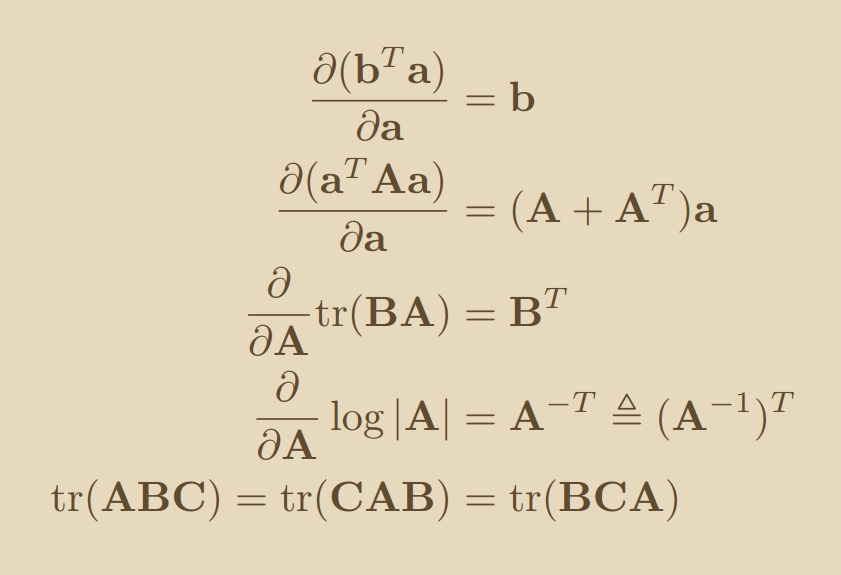
\includegraphics[width=\textwidth]{formulas.jpg}
    \caption{important formulas}
    \label{formulas1}
\end{figure}
\begin{labeling}{alligator}
\item [Mahalanobis distance] 
\item [Eigendecomposition:]
\item [Equation of Ellipse:] $(\mathbf{x - c})^T A (\mathbf{x - c})$
\item [Orthonormal Matrices:] $\mathbf{U}^T = \mathbf{U}^{-1} \Rightarrow  \mathbf{U}^{-T} = \mathbf{U}$
\item [Trace of a Matrix $A$:] $\textrm{tr}(A)=\sum _{i=1}^{n}a_{ii}=a_{11}+a_{22}+\dots +a_{nn}$
\item [Discriminant Analysi] $p(y=c | \mathbf{x, \theta}) = p(\mathbf{x} | y = c, \mathbf{\theta}) \times p(y = c | \mathbf{\theta})$
\end{labeling}
\end{document}
